\newcommand{\portadaA}{
    \thispagestyle{empty}
    \newgeometry{left=3cm,right=3cm}
    \noindent
    
\includegraphics[height = 2cm]{img/logoFCTo.png}

    \vspace{4cm}

    \begin{tcolorbox}[boxrule=0pt,frame hidden,colback=red!65]
 \ \\
 \begin{center}
 {\huge \textbf{\textcolor{white}{\thetitle}}}\\
 \ \\
 \ \\
 {\Large \textbf{\textcolor{white}{\mbox{Física del clima}}}}\\
 \ \\
 \ \\
 {\large \textbf{\textcolor{white}{\thedate}}}\\
 \medskip
 \end{center}
 \end{tcolorbox}

    \vfill
    \authorA\\
    \authorB\\
    \authorC\\
    \'Ultima versi\'on: \thedate
 
    \restoregeometry
    \newpage
}

\newcommand{\portadaB}{
\newgeometry{%
  paperwidth=210mm,%
  paperheight=297mm,%
  left=2mm,right=2mm,%
  top=2mm, bottom=2mm,%
  }
\thispagestyle{empty}
\noindent

\includegraphics[height=2.5cm]{img/logoFCTo.png}\\
\vspace{9cm}

\begin{tcolorbox}[boxrule=0pt,frame hidden,colback=black!65]
 \ \\
 \begin{center}
 {\huge \textbf{\textcolor{white}{\thetitle}}}\\
 \ \\
 \ \\
 {\Large \textbf{\textcolor{white}{\mbox{Física del clima}}}}\\
 \ \\
 \ \\
 {\large \textbf{\textcolor{white}{\thedate}}}\\
 \medskip
 \end{center}
 \end{tcolorbox}

 \vspace{9cm}

 \begin{flushright}
     \authorA\hspace{2cm}\mbox{}\\
     \authorB\hspace{2cm}\mbox{}\\
     \authorC\hspace{2cm}\mbox{}\\
     \authorD\hspace{2cm}\mbox{}\\
     \authorE\hspace{2cm}\mbox{}
     \end{flushright}
 \cleardoublepage
 \restoregeometry
}

\newcommand{\portadaC}{
\newgeometry{%
  paperwidth=210mm,%
  paperheight=297mm,%
  left=2mm,right=2mm,%
  top=2mm, bottom=2mm,%
  }
\thispagestyle{empty}
\noindent

\begin{textblock*}{12cm}(2cm,4cm)
\begin{tcolorbox}[boxrule=5pt,colback=yellow!45!blue,colframe=green!70!black]
 \ \\
 \begin{center}
 {\huge \textbf{\textcolor{white}{\thetitle}}}\\
 \ \\
 {\large \textbf{\textcolor{white}{Siglo XVII}}}\\
 \bigskip
 \end{center}
\end{tcolorbox}
\end{textblock*}


\begin{textblock*}{8cm}(7cm,14cm)
\includegraphics[width=\textwidth]{img/random.jpg}
\end{textblock*}
\begin{textblock*}{8cm}(5cm,12cm)
     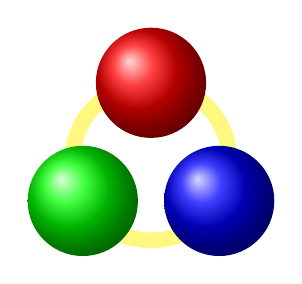
\begin{tikzpicture}
\path[fill=yellow!50!white] (0,0) circle (11mm);
\path[fill=white] (0,0) circle (9mm);
\foreach \w/\c in {90/red,210/green,330/blue}
{\path[shading=ball,ball color=\c] (\w:1cm) circle (7mm);}
\end{tikzpicture}
\end{textblock*}


\begin{textblock*}{5cm}(14cm,25cm)
     \begin{flushleft}
     \authorA\\
     \authorB
     \end{flushleft}
\end{textblock*}
 \cleardoublepage
\restoregeometry
}

\newcommand{\contraportadaA}{
\newgeometry{%
  paperwidth=210mm,%
  paperheight=297mm,%
  left=2mm,right=2mm,%
  top=2mm, bottom=2mm,%
  }
\thispagestyle{empty}
\begin{landscape}
\begin{tcolorbox}[boxrule=0pt,frame hidden,colback=red!65]
\ \\
\ \\
\ \\
\ \\
\ \\
\ \\
\ \\
\end{tcolorbox}
\end{landscape}
\restoregeometry
}

\newcommand{\contraportadaB}{
\newgeometry{%
  paperwidth=210mm,%
  paperheight=297mm,%
  left=2mm,right=2mm,%
  top=2mm, bottom=2mm,%
  }
\thispagestyle{empty}
\begin{landscape}
\ \\
\vspace{7cm}
\begin{tcolorbox}[boxrule=0pt,frame hidden,colback=yellow!50!black]
\ \\
\vspace{2cm}
\ \\
\end{tcolorbox}
\end{landscape}
\restoregeometry
}

\newcommand{\contraportadaC}{
\newgeometry{%
  paperwidth=210mm,%
  paperheight=297mm,%
  left=2mm,right=2mm,%
  top=2mm, bottom=2mm,%
  }
\thispagestyle{empty}
\ \\
\vspace{12cm}
\\
\begin{tcolorbox}[boxrule=0pt,frame hidden,colback=blue!65]
\ \\
\vspace{2cm}
\ \\
\end{tcolorbox}
\restoregeometry
}